
\documentclass[a4paper,11pt]{article}

\usepackage[T1]{fontenc}
\usepackage{fancyhdr}
\pagestyle{fancy}
\usepackage{ae}
\usepackage[latin1]{inputenc}
\usepackage[brazil]{babel}
\usepackage[brazil]{hyperref}
\usepackage[alf]{abntex2cite}
\usepackage{listings}

\usepackage{graphicx}
\usepackage{url}
\usepackage{lastpage}
\usepackage{multirow}
\usepackage{indentfirst}
\usepackage{amsmath}
\usepackage{siunitx}
\usepackage{booktabs}
\usepackage{pgfplots}
\usepackage{tikz}
\usepgfplotslibrary{colormaps} 
\usepackage{xifthen}
% \usepackage[miktex]{gnuplottex}
%\usepackage{gnuplottex}

\usepackage{subfloat}
\usepackage{float} 
\usepackage{subfig}
\usepackage{varwidth}
\newcommand{\subfigref}[1]{\hyperref[#1]{Figura~\ref*{#1}}}

\sisetup{output-decimal-marker = {,}}
\newcommand{\theauthori}{}
\newcommand{\theauthorii}{}
\newcommand{\theauthoriii}{}
\renewcommand{\title}[1]{\newcommand{\thetitle}{#1}}
\renewcommand{\author}[1]{\newcommand{\theauthor}{#1}}
\newcommand{\authori}[1]{\renewcommand{\theauthori}{#1}}
\newcommand{\authorii}[1]{\renewcommand{\theauthorii}{#1}}
\newcommand{\authoriii}[1]{\renewcommand{\theauthoriii}{#1}}
\newcommand{\class}[1]{\newcommand{\theclass}{#1}}
\newcommand{\classProffessor}[1]{\newcommand{\theclassProffessor}{#1}}
\usepackage{palatino}
\renewcommand{\textsc}[1]{\fontshape{sc} \fontfamily{\sfdefault} \selectfont #1}

\mathchardef\period=\mathcode`.
\DeclareMathSymbol{.}{\mathord}{letters}{"3B}
\DeclareMathOperator{\erf}{erf}
\DeclareMathOperator{\diff}{d}

\allowdisplaybreaks
\newenvironment{conditions}[1][]
  {#1 \begin{tabular}[t]{>{$}r<{$} @{${}={}$} l @{$\quad$}r @{  }l}}
  {\end{tabular}\\}

  \usetikzlibrary{shapes,shadows}
  \tikzstyle{exercisebox} = [draw=black, rectangle, 
  inner sep=10pt, style=rounded corners, drop shadow={fill=gray,
  opacity=1}]
  \tikzstyle{exercisetitle} =[fill=white]
 \newcommand{\boxexercise}[2]{ 
    \begin{center}
      \begin{tikzpicture}
        \node [exercisebox, fill=black!1!] (box)
        {\begin{minipage}{0.9\textwidth}
            \setlength{\parindent}{1em}
            \footnotesize  \vspace{\belowdisplayskip} #2
          \end{minipage}};
        \node[exercisetitle, right=10pt, draw=black, style=rounded corners] at
        (box.north west) {Exerc�cio: #1};
      \end{tikzpicture}
    \end{center}
  }

  \tikzstyle{examplebox} = [draw=black, rectangle, 
  inner sep=10pt, style=rounded corners, drop shadow={fill=gray,
  opacity=1}]
  \tikzstyle{exampletitle} =[fill=white]
 \newcommand{\boxexample}[2]{ 
    \begin{center}
      \begin{tikzpicture}
        \node [examplebox, fill=green!10!] (box)
        {\begin{minipage}{0.9\textwidth}
            \setlength{\parindent}{1em}
            \footnotesize \vspace{\belowdisplayskip} #2
          \end{minipage}};
        \node[exampletitle, right=10pt, draw=black, style=rounded corners] at
        (box.north west) {Exemplo: #1};
      \end{tikzpicture}
    \end{center}
  }

\onehalfspacing
\newcommand{\code}[1]{\texttt{#1}}

\renewcommand{\lstlistingname}{C�digo}
\lstset{ language=Matlab,
  basicstyle=\ttfamily,
  basicstyle=\fontfamily{pcr}\fontseries{m}\selectfont\footnotesize,
  breaklines=true,
  columns=fullflexible,
  commentstyle=\color[rgb]{0,0.5,0},
  numbers=left,
  showstringspaces=false,
  morekeywords={matlab2tikz},
  keywordstyle=\color{blue},%
  numberstyle=\tiny\sffamily\color{black},
  frame=tb,
  stringstyle=\color[rgb]{0.5,0,0.5},
  numberstyle=\fontfamily{pcr}\fontseries{m}\selectfont\tiny,
  aboveskip=10pt,belowskip=20pt,
  }

\usepackage{fancyvrb}
% redefine \VerbatimInput
\RecustomVerbatimCommand{\VerbatimInput}{VerbatimInput}%
{fontsize=\scriptsize,frame=single,
rulecolor=\color{lightgray!80},
}

% o novo maketitlepage
\renewcommand{\maketitle}{
% Primeira p�gina de t�tulo  
\pagestyle{empty}
\begin{center}   
\textsc \large  
Universidade Federal do Rio Grande do Sul \\
Escola de Engenharia \\
Departamento de Engenharia Qu�mica \\
Programa de P�s--Gradua��o em Engenharia Qu�mica
\vfill
\Large \textsc \theclass \\ Prof:~\theclassProffessor
\vfill \vfill
\huge \bfseries \textsc  
\thetitle
\vfill \vfill
\begin{varwidth}[t]{\textwidth}
\Large \bfseries \textsc 
\theauthor\\
\ifthenelse{\equal{\theauthori}{}}{}{\theauthori\\}
\ifthenelse{\equal{\theauthorii}{}}{}{\theauthorii\\}
\ifthenelse{\equal{\theauthoriii}{}}{}{\theauthoriii}
\end{varwidth}
\vfill \vfill
\large \textsc Porto Alegre, RS \\ \today
\end{center}
\clearpage
\setcounter{page}{1}
\pagestyle{fancy}
\lhead{}
} % end maketitle 


% \usepackage[miktex]{gnuplottex} %Windows
%\usepackage{gnuplottex} %Ubuntu

\begin{document} 
\class{EQP 0026--Otimiza��o de Processos}
\classProffessor{Marcelo Farenzena}
% \classProffessorii{Fulano 1}
% \classProffessoriii{Fulano 2}
% \classProffessoriv{Fulano 3}

\author{Guilherme Braganholo Fl�res
\center{\normalsize{00170787}}}
% \authorii{Fulano 1}
% \authoriii{Fulano 2}
% \authoriv{Fulano 3}

\title{
% Convexidade
% \\ Pontos de M�nimo e M�ximo
% Otimiza��o sem Restri��es
Compara��o de m�todos de otimiza��o global aplicado � par�metros do modelo
F--SAC.
% \\ Trab
% \\ Trab
% \\ Trab
% \\ Trab
% \\ Trab
% \\ Trab
% \\ Trab
% \\ Trab
% \\ Trab
}
\titlemin{Trabalho~Final}
 
\maketitle 
 
% \section*{Defini��es importantes} 
\begin{equation*} 
\renewcommand{\arraystretch}{2.5}
\begin{aligned}
f(x)& = \text{polinomio em fun��o do vetor }x  \\ \\
\nabla f(x) &= \left[
\begin{array}{c}
\cfrac{\partial f}{\partial x_1}\\
\cfrac{\partial f}{\partial x_2}\\
\vdots\\
\cfrac{\partial f}{\partial x_n}\\
\end{array}
\right]\\ \\
\nabla^2 f(x) &= \left[
\begin{array}{cccc}
\cfrac{\partial^2 f}{\partial x_1 \partial x_1} 
& \cfrac{\partial^2 f}{\partial x_1 \partial x_2} & \cdots
& \cfrac{\partial^2 f}{\partial x_1 \partial x_n}\\
\cfrac{\partial^2 f}{\partial x_2 \partial x_1} 
& \cfrac{\partial^2 f}{\partial x_2 \partial x_2} & \cdots
& \cfrac{\partial^2 f}{\partial x_2 \partial x_n}\\
\vdots & \vdots & \ddots
& \vdots\\
\cfrac{\partial^2 f}{\partial x_n \partial x_1} 
& \cfrac{\partial^2 f}{\partial x_n \partial x_2} & \cdots
& \cfrac{\partial^2 f}{\partial x_n \partial x_n}\\
\end{array}
\right]
\end{aligned}
\end{equation*}
\clearpage

\section {Convexidade}
Analisar a convexidade das seguintes fun��es objetivo:
\begin{align}
f_1 (x) &= 2x_1 + 3x_2 +6 \label{eq:1f1}\\ 
f_2 (x) &= x_1^3 \label{eq:1f2}\\
f_3 (x) &= x_1^2 + x_1 x_2 + x_2 + 4 \label{eq:1f3}
\end{align}

\subsection*{\autoref{eq:1f1}}
\begin{equation}
f_1 (x) = 2x_1 + 3x_2 +6 \tag{\ref{eq:1f1}}
\end{equation}
Para a \autoref{eq:1f1} temos que o gradiente de $f_1(x)$ � dado por:
\begin{equation}
\nabla f_1(x) = \left[
\begin{array}{c}
2\\
3
\end{array}
\right]
\end{equation}
e para a hessiana temos:
\begin{equation}
\nabla^2 f_1(x) = \left[
\begin{array}{cc}
0& 0\\
0& 0
\end{array}
\right]
\end{equation}

Calculando os autovalores da matriz $\nabla^2 f_1(x)$ temos para $\forall x$:
\begin{itemize}
  \item $\lambda_1 = 0$
  \item $\lambda_2 = 0$
\end{itemize}
portanto temos uma fun��o convexa, neste caso um plano, dado que a fun��o �
linear.


\subsection*{\autoref{eq:1f2}}
\begin{equation}
f_2 (x) = x_1^3 \tag{\ref{eq:1f2}}
\end{equation}
Para a Equa��o \autoref{eq:1f2} temos que o gradiente de $f_2(x)$ � dado por:
\begin{equation}
\nabla f_2(x) = \left[
\begin{array}{c}
3x_1^2
\end{array}
\right]
\end{equation}
e para a hessiana temos:
\begin{equation}
\nabla^2 f_2(x) = \left[
\begin{array}{c}
6x_1
\end{array}
\right]
\end{equation}

Calculando os autovalores da matriz $\nabla^2 f_2(x)$ temos:
\begin{itemize}
  \item $\lambda_1 = \left\{
\begin{array}{ccc}
\geq 0& \rm{se}& x_1 \geq 0\\
\leq 0& \rm{se}& x_1 \leq 0
\end{array}
\right.$
\end{itemize}
portanto temos uma fun��o convexa para valores positivos de $x_1$ e n�o convexa
para valores de $x_1$ menores que $0$.
\begin{figure}[h]
\centering
\def\FunctionF(#1){(#1)^3}
\def\FunctionFd(#1){3*(#1)^2}
\def\FunctionFdd(#1){6*(#1)}
\subfloat[$f_1(x)$]{
\begin{tikzpicture}[scale=0.8]
\begin{axis}[
        axis y line=center,
        axis x line=middle, 
        axis on top=true,
    ]
    \addplot [domain=-2:2, samples=51, mark=none, ultra thick, blue] {\FunctionF(x)};
    \node [right, blue] at (axis cs: 0.5,4.5) {$f_2(x)$};
\end{axis}
\end{tikzpicture}}
\hfill
\subfloat[$\nabla f_1(x)$]{
\begin{tikzpicture}[scale=0.8]
\begin{axis}[
        axis y line=center,
        axis x line=middle, 
        axis on top=true,
    ]
    \addplot [domain=-2:2, samples=51, mark=none, ultra thick, orange]
    {\FunctionFd(x)};
	\addplot [domain=-2:2, samples=51, mark=none, ultra thick, red]
	{\FunctionFdd(x)};
\node [right, orange] at (axis cs: 0.5,-5) {$\nabla f_2(x)$};
\node [right, red] at (axis cs: 0.5,-7) {$\nabla^2 f_2(x)$};
\end{axis}
\end{tikzpicture}}
\caption{$f_2(x) = x_1^3$.}
\label{fig:1f2}
\end{figure}



\subsection*{\autoref{eq:1f3}}
\begin{equation}
f_3 (x) = x_1^2 + x_1 x_2 + x_2 + 4  \tag{\ref{eq:1f3}}
\end{equation}
Para a Equa��o \autoref{eq:1f3} temos que o gradiente de $f_3(x)$ � dado por:
\begin{equation}
\nabla f_3(x) = \left[
\begin{array}{c}
2x_1 + x_2 \\
x_1 + 2
\end{array}
\right]
\end{equation}
e para a hessiana temos:
\begin{equation}
\nabla^2 f_3(x) = \left[
\begin{array}{cc}
2 & 1\\
1 & 0
\end{array}
\right]
\end{equation}

Calculando os autovalores da matriz $\nabla^2 f_3(x)$ temos para $\forall x$:
\begin{itemize}
  \item $\lambda_1 = 1 + \sqrt{2} = 2.41$
  \item $\lambda_2 = 1 - \sqrt{2} = -0.41$
\end{itemize}

Sendo esta matriz n�o definida, n�o � uma fun��o convexa.

\clearpage
\section {Pontos de M�nimo e M�ximo}
Analisar pontos de m�ximo e m�nimo das seguintes fun��es:
\begin{align}
f_1 (x) &= |x| \label{eq:2f1}\\ 
f_2 (x) &= -x_1^4 + x_1^3 +20 \label{eq:2f2}\\
f_3 (x) &= x_1^2 + 2x_1 + 3x_2^2 + 6x_2 + 2 \label{eq:2f3}
\end{align}

\subsection*{\autoref{eq:2f1}}
\begin{equation}
f_1 (x) = |x| \tag{\ref{eq:2f1}} 
\end{equation}
Para a Equa��o \autoref{eq:2f1} temos que o gradiente de $f_1(x)$ � dado por:
\begin{equation}
\nabla f_1(x) = \left[
\begin{array}{cc}
1 &\quad \text{se } x> 0\\
-1 &\quad \text{se } x < 0
\end{array}
\right]
\end{equation}

Aplicando em $x_1 = 0$ temos $f_1(x) = 0$ e para $\forall$ valores de $x$
aplicados em $f_1(x)$ s�o obtidos valores maiores que $0$, como podemos observar
na \autoref{fig:2f1}:
\begin{figure}[h]
\centering
\def\FunctionF(#1){abs(#1)}
\def\FunctionFd(#1){1}
\def\FunctionFdd(#1){-1}
\subfloat[$f_1(x)$]{
\begin{tikzpicture}[scale=0.8]
\begin{axis}[
        axis y line=center,
        axis x line=middle, 
        axis on top=true,
        xmin=-5,
        xmax=5,
        ymin=0,
        ymax=5,
    ]
    \addplot [domain=-5:5, samples=51, mark=none, ultra thick, blue] {\FunctionF(x)};
    \node [right, blue] at (axis cs: 0.5,4.5) {$f_1(x)$};
\end{axis}
\end{tikzpicture}}
\hfill
\subfloat[$\nabla f_1(x)$]{
\begin{tikzpicture}[scale=0.8]
\begin{axis}[
        axis y line=center,
        axis x line=middle, 
        axis on top=true,
        xmin=-5,
        xmax=5,
        ymin=-1.2,
        ymax=1.2,
    ]
    \addplot [domain=0:5, samples=51, mark=none, ultra thick, orange]
    {\FunctionFd(x)};
	\addplot [domain=-5:0, samples=51, mark=none, ultra thick, orange]
	{\FunctionFdd(x)}; 
\node [right, orange] at (axis cs: 0.5,0.5) {$\nabla f_1(x)$};
\end{axis}
\end{tikzpicture}}
\caption{$f_1(x) = |x|$.}
\label{fig:2f1}
\end{figure}

Portanto podemos concluir que temos um ponto de m�nimo, apesar do gradiente de
$f_1(x)$ n�o ser cont�nuo e portanto nao ser poss�vel o calculo da hessiana de
$f_1(x)$.

\subsection*{\autoref{eq:2f2}}
\begin{equation}
f_2 (x) = -x_1^4 + x_1^3 +20 \tag{\ref{eq:2f2}} 
\end{equation}
Para a Equa��o \autoref{eq:2f2} temos que o gradiente de $f_2(x)$ � dado por:
\begin{equation}
\nabla f_2(x) = \left[
\begin{array}{c}
-4x_1^3 + 3x_1^2
\end{array}
\right]
\end{equation}
Para um ponto de m�nimo ou m�ximo devemos obter $\nabla f_2(x) = 0$, o que
ocorre quando:
\begin{itemize}
  \item $x_1 = 0$
  \item $x_1 = \cfrac{3}{4}$
\end{itemize}
portanto devemos analizar o valor da hessiana nestes dois pontos, como �
poss�vel observar na \autoref{fig:2f2}.

\begin{figure}[h]
\centering
\def\FunctionF(#1){-(#1)^4 + (#1)^3 +20}
\def\FunctionFd(#1){-4*(#1)^3 + 3*(#1)^2}
\def\FunctionFdd(#1){-12*(#1)^2 + 6*(#1)}

\subfloat[$f_2(x)$]
{\begin{tikzpicture}[scale=0.8]
\begin{axis}[
        axis y line=center,
        axis x line=middle, 
        axis on top=true,
        xmin=-1,
        xmax=1.5,
        ymin=19,
        ymax=21,
    ]
    \addplot [domain=-2:2.5, samples=100, 
    mark=none, ultra thick, blue]{\FunctionF(x)};
\node [right, blue] at (axis cs: 0.5,20.5) {$f_2(x)$};
\end{axis}
\end{tikzpicture}}
\subfloat[$\nabla f_2(x)$ e $\nabla^2 f_2(x)$]
{\begin{tikzpicture}[scale=0.8]
\begin{axis}[
        axis y line=center,
        axis x line=middle, 
        axis on top=true,
        xmin=-1,
        xmax=1,
        ymin=-1,
        ymax=2,
    ]
    \addplot [domain=-2:2.5, samples=100, 
    mark=none, ultra thick, orange]{\FunctionFd(x)};
    \addplot [domain=-2:2.5, samples=100, 
    mark=none, ultra thick, red]{\FunctionFdd(x)};
\node [right, orange] at (axis cs: 0.1,1.5) {$\nabla f_2(x)$};
\node [right, red] at (axis cs: 0.1,1.0) {$\nabla^2 f_2(x)$};
\end{axis}
\end{tikzpicture}}
\caption{$f_2 (x) = -x_1^4 + x_1^3 +20$.}
\label{fig:2f2}
\end{figure}

A hessiana de $f_2(x)$ � dada por:
\begin{equation}
\nabla^2 f_2(x) = \left[
\begin{array}{c}
-12x_1^2 + 6x_1
\end{array}
\right]
\end{equation}

Aplicada em $x_1 = 0$ em $\nabla f_2(x)$ temos:
\begin{equation}
\nabla^2 f_2(0) = \left[
\begin{array}{c}
0
\end{array}
\right]
\end{equation}
onde n�o podemos concluir se � um ponto de m�ximo ou m�nimo, pois � uma matriz
indefinida, o que leva a creer que seja um ponto de inflex�o. Isto pode ser
observando na \autoref{fig:2f2} onde � apresentado o comportamento da fun��o
$f_2(x)$.

Aplicada em $x_1 = \cfrac{3}{4}$ em $\nabla f_2(x)$ temos:
\begin{equation}
\nabla^2 f_2 \left(\frac{3}{4}\right) = \left[
\begin{array}{c}
-2.25
\end{array}
\right]
\end{equation}
onde podemos concluir diretamente, pelo autovalor �nico $(\lambda_1 = -2.25)$,
que se trata de um ponto de m�ximo, para este caso.

\subsection*{\autoref{eq:2f3}}
\begin{equation}
f_3 (x) = x_1^2 + 2x_1 + 3x_2^2 + 6x_2 + 2 \tag{\ref{eq:2f3}} 
\end{equation}
Para este �ltimo caso, temos $\nabla f_3(x)$ dado por:
\begin{equation}
\nabla f_3(x) = \left[
\begin{array}{c}
2x_1 + 2\\
6x_2 + 6
\end{array}
\right]
\end{equation}

Para a condi��o necess�ria de m�ximo ou minimos devemos ter $\nabla f_3(x) =
0$, isto ocorre apenas em $x = [-1, -1]^{\rm{T}}$. Partindo da hessiana de
$f_3(x)$ que � igual �:
\begin{equation}
\nabla^2 f_3(x) = \left[
\begin{array}{cc}
2 & 0\\
0& 6
\end{array}
\right]
\end{equation}
e aplicando em $x = [-1, -1]^{\rm{T}}$ temos os uma matriz positiva definida,
com os seguintes autovalores:
\begin{itemize}
  \item $\lambda_1 = 6$
  \item $\lambda_2 = 2$
\end{itemize}
portanto, um ponto de m�nimo.


% \newenvironment{conditions}[1][where:]
  {#1 \begin{tabular}[t]{>{$}r<{$} @{${}={}$} l @{$\quad$}r @{$\quad$}l}}
  {\end{tabular}\\[\belowdisplayskip]}
\section {Otimiza��o sem restri��es}
\newenvironment{answers}[1][The answers in the reference were:]
  {#1 \begin{tabular}[t]{>{$}r<{$} @{${}={}$} l}}
  {\end{tabular}\\[\belowdisplayskip]}
\subsection{Exerc�cio 6.48 \cite{edgar2001optimization} (p�gina 220)}
  
The cost of refined oil when shipped via the Malacca Straits to Japan in dollars
per kiloliter was given (Uchiyama, 1968) as the linear sum of the crude oil
cost, the insurance, customs, freight cost for the oil, loading and unloading
cost, sea berth cost, submarine pipe cost, storage cost, tank area cost,
refining cost, and freight cost of products as:
\begin{equation}
\begin{aligned}
c = c_c &+ c_i + c_x + \frac{2.09\times 10^{4} t^{-0.3017}}{360} + \frac{1.064
\times 10^{6} at^{0.4925}}{52.47q\left(360\right)} \\
&+ \frac{4.242 \times 10^{4} at^{0.7952} + 1.813 ip \left(nt + 1.2q
\right)^{0.861}}{52.47q\left(360\right)}\\
&+ \frac{4.25 \times 10^{3} a\left(nt+1.2q\right) }{52.47q\left(360\right)}
+ \frac{5.042 \times 10^{3} q^{-0.1899}}{360}\\
&+ \frac{0.1049q^{0.671}}{360}
\end{aligned}
\end{equation}
\begin{conditions}
a	& annual fixed charges	& {fraction}	&($0.20$) \\
c_c	& crude oil price		&{\$/kL}		&($12.50$)\\
c_i	& insurance cost		&{\$/kL}		&($0.50$)\\
c_x	& customs cost			&{\$/kL}		&($0.90$)\\
i	& interest rate			&				&($0.10$)\\
n	& number of ports		&				&($2$)\\
p	& land price			&{\$/m$^2$}		&($7000$)\\
q	& refinery capacity		&{bbl/day}		&\\
t	& tanker size			&{kL} 			&\\
\end{conditions}
Given the values indicated in parentheses, use a computer code to compute the
minimum cost of oil and the optimum tanker size $t$ and refinery size $q$ by
Newton's method and the quasi-Newton method (note that $1~\text{kL} = 6.29
~\text{bbl}$).

\begin{answers}{}
t & $427000$ dwt $\approx$ $485000$ kL \\
q & $185000$ bbl/day
\end{answers}

\noindent\makebox[\linewidth]{\rule{\textwidth}{0.4pt}}
\subsubsection{Newton}
bla
\subsubsection{quasi-Newton}
bla  

\clearpage

\subsection{Exerc�cio 6.44 \cite{edgar2001optimization} (p�gina 219)}
In a decision problem it is desired to minimize the expected risk defined as
follows: 
\begin{equation}
\varepsilon \{\text{risk} \} = \left(1-P\right)c_1\left[1-F(b) \right] + P c_2
\theta
\left(\frac{b}{2}+\frac{2\pi}{4}\right)F\left(\frac{b}{2}-\frac{\sqrt{2\pi}}{4}\right)
\end{equation}
\begin{conditions}
F(b) & $\displaystyle\int_{-\infty}^b e^{-u^2 / 2\theta^2} \text{d}u$ (normal
probability function)\\
c_1 & $1.25\times10^{5}$\\
c_2& $15$\\
\theta & $2000$\\
P &$0.25$
\end{conditions}
Find the minimum expected risk and $b$. 

\noindent\makebox[\linewidth]{\rule{\textwidth}{0.4pt}}

bla


\clearpage
\subsection{Exerc�cio Antoine - Etanol}
bla

 
% 
\section {Lista 2 -- Otimiza��o sem restri��o}

Objetivo: Avaliar os m�todos de otimiza��o sem restri��es, tanto de busca quanto
de m�trica vari�vel, para uma s�rie de fun��es objetivos.

M�todos:
\begin{itemize}
  \item Busca (DFO) -- Simplex, Hooke e Jeeves e Powell;
  \item Gradiente -- M�xima descida e gradientes conjugados (\code{cgrad});
  \item Quase-Newton -- BFGS e DFP;
  \item Newton -- Newton e Levenberg Marquard (\code{lmarqua})
\end{itemize}
\boxexercise{1}
{ 
Tabela com comparativo dos diferentes m�todos para os diferentes
problemas. Deve-se executar cada algoritmo 100 vezes, com diferentes chutes
iniciais gerados aleatoriamente. Hierarquizar os m�todos e elencar os tr�s
melhores no geral. Atente que dentro do arquivo .m h� a resposta de cada teste.
Utilize duas pol�ticas para chute inicial - uma de menor raio e outra de maior.
}

A avalia��o dever� contemplar as seguintes m�tricas, para cada algoritmo $i$:

Efic�cia ($\theta_i$):
\begin{equation}
\theta_i = \frac{100}{N}\sum_{j=1}^{N}\frac{T^*_j}{T_{i, j}}
\end{equation}

Efici�ncia ($\chi_i$)
\begin{equation}
\chi_i = \frac{100}{N}\sum_{j=1}^{N}\frac{S^*_j}{S_{i, j}}
\end{equation}

Robustez ($\eta_i$)
\begin{equation}
\eta_i = 100\frac{N_i}{N}
\end{equation}

Qualidade da solu��o obtida ($\xi_i$)
\begin{equation}
\xi_i = \frac{100}{N}\sum_{j=1}^{N}\frac{\left(d^*_j + \varepsilon
\right)}{\left(d_{i, j} + \varepsilon \right)}
\end{equation}

Onde $T_{i, j}$ � o seu tempo computacional para resolver o problema $j$,
$T_j^*$ � o menor tempo entre os algoritmos para resolver o problema $j$,
$S_{i,j}$ � o seu n�mero de avalia��es da fun��o objetivo para resolver o
problema $j$, $S_j^*$ � o menor n�mero de avalia��es entre os algoritmos para
resolver o problema $j$, $d_j^*$ � a melhor qualidade da solu��o para o problema
$j$, $d_{i,j}$ � a qualidade da solu��o para o problema $j$ definida como:
\begin{equation}
d_{i, j} = \frac{\left \| x_{i, j} - x_j^* \right \|}{\varepsilon_x}
+\frac{\left | S(x_{i, j}) - S(x_j^*) \right |}{\varepsilon_S}
\end{equation}
onde�$\varepsilon$�� a precis�o da m�quina,�$\varepsilon_x$ � a toler�ncia na 
vari�vel independente,�$\varepsilon_S$ � a toler�ncia na fun��o objetivo,
$x_j^*$ � a solu��o exata do problema $j$, $N_i$ � o seu n�mero de problemas resolvidos
e $N$ � o n�mero total de problemas. Quando o $i$-�simo algoritmo n�o consegue
resolver o $j$-�simo problema, ent�o $T_{i, j} = \infty$�e $S_{i, j} = \infty$.

Pol�tica do chute inicial: gerar $100$ diferentes chutes iniciais rand�micos
(uniformemente distribu�dos) para cada problema. Usar o mesmo conjunto de $100$
chutes para os diferentes m�todos. Devem ser utilizados dois conjuntos de
valores lim�trofes para os chutes $[0\;\ 2]$ e $[-2\;\ 4]$.

Software: MATLAB
Arquivos: baixar do Moodle os arquivos problemas.zip e algoritmos.zip e extrai-los no mesmo
diret�rio.

\boxexercise{2}
{
Algoritmo pr�prio (proposto pelo aluno, ou em dupla) que tenha performance
compar�vel aos tr�s melhores.}

\subsection {Introdu��o}
Foram executados apenas os algoritmos \code{hkjeeves}, \code{cgrad},
\code{newton} e \code{lmarqua}, os demais m�todos de otimiza��o
\code{ccomplex}, \code{steepdes}, \code{bfgs} e \code{dfp}, apresentaram erros
na execu��o de todos os problemas.

Obs.: O m�todo \code{ccomplex} est� com o nome do arquivo diferente do nome da
fun��o do mesmo nos arquivos disponibilizados no Moodle.

\subsection {Resolu��o dos problemas}
Para a resolu��o do exerc�cio, foi implementado o \autoref{code:script},
presente no \autoref{ap:trab3}, em Matlab\textsuperscript{\textregistered}. Em
um �nico c�digo foi poss�vel executar os $13$ problemas propostos utilizando os
$4$ m�todos poss�veis. Por fim, este c�digo tamb�m contempla o c�lculo da Efic�cia
($\theta$) Efici�ncia ($\chi$), Robustez ($\eta$) e Qualidade da solu��o obtida
($\xi$) para cada m�todo utilizado.

\subsection {Resultados} 
Os m�todos foram ranqueados pela soma dos valores de todas as m�trica utilizadas
neste trabalho, sendo o maior valor o melhor m�todo e o menor valor o pior. 
Devido a mera coincid�ncia da ordem de execu��o, os m�todos apresentados nas
Tabelas \ref{tab:res1} e \ref{tab:res2} j� est�o ranqueados.

\begin{table}[H]
\renewcommand{\arraystretch}{1.1}
\sisetup{table-format=3.4,round-mode=places,round-precision=4}
\caption{Resultados obtidos com cada m�todo para os problemas propostos
utilizando a pol�tica de chutes iniciais com valores no intervalo de $[0\;\ 2]$.}
\label{tab:res1}
\footnotesize
\begin{center}
\begin{tabular}{lSSSSS}
\toprule
\multirow{2}{*}{M�todo}& {Efic�cia}& {Efici�ncia} & {Robustez} & {Qual. sol.}
&\multicolumn{1}{c}{\multirow{2}{*}{Total}}\\
& {$\theta$} & {$\chi$} & {$\eta$} & {$\xi$}&\\
\midrule
\code{hkjeeves}	&	39,89972997	&	50,38098074	&	100.	&	13,30526098	&	203,5859717
\\
\code{cgrad}	&	38,18960345	&	35,97782424	&	92,30769231	&	8,000048048	&	174,4751681	\\
\code{newton}	&	22,41874463	&	14,87457198	&	38,46153846	&	15,38463975	&	91,13949482	\\
\code{lmarqua}	&	13,8153285	&	16,67904777	&	38,46153846	&	7,700211197	&	76,65612593	\\
\bottomrule
\end{tabular}
\end{center}
\end{table} 

\begin{table}[H]
\renewcommand{\arraystretch}{1.1}
\sisetup{table-format=3.4,round-mode=places,round-precision=4}
\caption{Resultados obtidos com cada m�todo para os problemas propostos
utilizando a pol�tica de chutes iniciais com valores no intervalo de $[-2\;\
4]$.}
\label{tab:res2}
\footnotesize
\begin{center}
\begin{tabular}{lSSSSS}
\toprule
\multirow{2}{*}{M�todo}& {Efic�cia}& {Efici�ncia} & {Robustez} & {Qual.sol.}
&\multicolumn{1}{c}{\multirow{2}{*}{Total}}\\
& {$\theta$} & {$\chi$} & {$\eta$} & {$\xi$}&\\
\midrule
\code{hkjeeves}	&	36,59551938	&	48,54099766	&	100.	&	17,17011135	&	202,3066284 \\
\code{cgrad}	&	26,35520142	&	30,02923131	&	69,23076923	&	7,694121386	&	133,3093233	\\
\code{newton}	&	17,32331114	&	13,21723285	&	30,76923077	&	15,38462484	&	76,69439959	\\
\code{lmarqua}	&	8,041719122	&	8,174684847	&	15,38461538	&	7,692307692	&	39,29332705	\\
\bottomrule
\end{tabular}
\end{center}
\end{table} 











 



\boxabstract{
Escrever o resumo aqui.
}

\section {Introdu��o}
O crescimento cont�nuo da demanda de energia tamb�m gera um crescimento no
consumo de combust�veis f�sseis. Entretanto, sabemos que este � um recurso
finito, fazendo com que diversos pesquisadores busquem diferentes formas de
diversificar a matriz energ�tica. Dentre as solu��es procuradas, deseja-se que
seja ambientalmente correta, ou seja:
\begin{itemize}
  \item Renov�vel;
  \item Baixo impacto abiental;
  \item Baixo custo.
\end{itemize}

Uma das alternativas bastante estudadas � o bio-etanol, um combust�vel l�quido
e que pode ser obtido de a partir de diversas mat�rias primas em diferentes
processos. Entre os processos existentes para a produ��o de etanol, o mais
utilizado � via fermenta��o, seja de cana de a��car, beterraba ou milho. Porem
este processo envolve grande quantidade de �gua, pois os micro-organismos
respons�veis pela transforma��o da glicose em etanol n�o s�o t�o resistentes
quanto se desejaria.

Motivado por este problema energ�tico, temos que, o conhecimento do
comportamento do equil�brio liquido-vapor do sistema etanol �gua � de suma
import�ncia para a ind�stria alcooleira. Um dos principais motivos para esta
preocupa��o � o uso na gasolina. O �lcool incorporado na gasolina deve ser do
tipo \emph{anidro} (sem �gua), por�m, sabemos que o sistema etanol �gua forma um
aze�tropo positivo com rela��o � press�o para sistemas isot�rmicos em
temperaturas moderadas (negativo com rela��o � temperatura em situa��es
isob�ricas para press�o moderada). Este aze�tropo pode ser melhor observado na
\autoref{fig:vle1}.
\begin{figure}[H]
\centering
{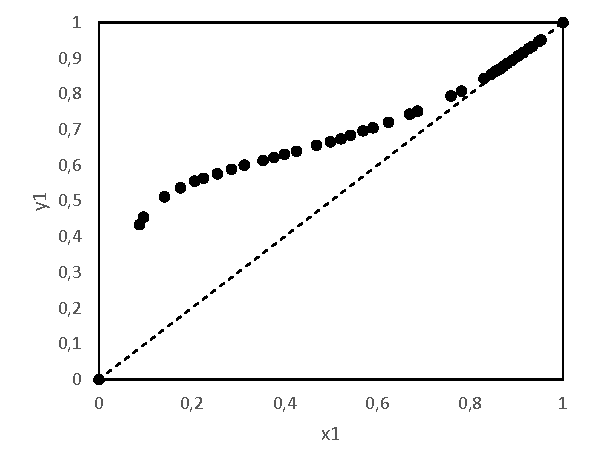
\includegraphics[width=0.45\textwidth]
{trabFinal/EtOH1.pdf}}
{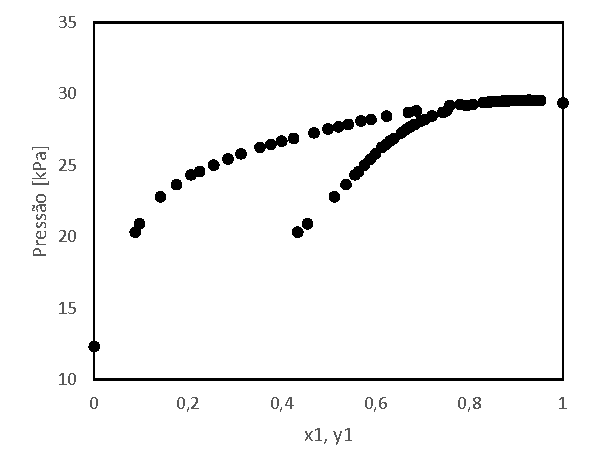
\includegraphics[width=0.45\textwidth]
{trabFinal/EtOH2.pdf}}
\caption{Comportamento do equil�brio l�quido vapor da mistura etanol (1) �gua
(2) na temperatura de $323.15$~K, onde � poss�vel observar o aze�tropo. Dados
experimentais de \citeonline{Kurihara1995}}
\label{fig:vle1}
\end{figure}

O aze�tropo formado por esta mistura impossibilita a separa��o do etanol puro
em uma coluna de destila��o simples. \citeonline{Haelssig2008} estudou a
obten��o do etanol anidro obtido pelo processo de fermenta��o com diversas
configura��es de colunas e em diferentes press�es de opera��o buscando o �timo
econ�mico. Segundo seu trabalho, o melhor economicamente e mais fact�vel foi a
configura��o de duas colunas operando em s�rie com press�es distintas. O
trabalho de \citeonline{Haelssig2008} corroborou com a os resultados obtidos
por \citeonline{Larsson1996}.

Para que seja poss�vel obter o comportamento confi�vel do equil�brio
l�quido-vapor algum tipo de sistema (bin�rio ou multicomponente) para o uso em
simula��es nas etapas de projeto e/ou otimiza��o de processos de separa��o, como
por exemplo a destila��o, s�o necess�rios dados de equil�brio confi�veis e um
modelo de coeficiente de atividade da fase l�quida (modelo de $\gamma_i$ ou
tamb�m conhecido como modelo de $g^{\rm{E}}$) robusto o suficiente para o
sistema em quest�o.

Uma grande quantidade de dados de equil�brio l�quido-vapor (VLE, Vapor-Liquid
Equilibrium) para o sistema etanol/�gua est�o dispon�veis na literatura. Assim
como diversos modelos de $g^{\rm{E}}$ e modelos de outras propriedades
termodin�micas para este mesmo sistema. Como descrito por
\citeonline{Haelssig2008} os modelos dispon�veis como Wilson e UNIQUAC ora
falham na predi��o do aze�tropo ora s�o incapazes de prover informa��es
energ�ticas da mistura, como entalpia de mistura. No seu trabalho,
\citeonline{Haelssig2008} prop�e como um dos objetivos de seu trabalho o
desenvolvimento de uma nova depend�ncia com a temperatura para modelos de
$g^{\rm{E}}$ (UNIQUAC, Wilson e NRTL) comuns em simuladores de processos em que
se utilizam intera��es bin�rias, utilizando dados de VLE, pontos de aze�tropo e
entalpia de excesso ($h^{\rm{E}}$).

O objetivo deste trabalho � a reprodu��o do trabalho de
\citeonline{Haelssig2008}, por�m verificando a capacidade do modelo F-SAC+Disp
\citeonline{Flores2016} com os mesmos tipos de dados experimentais (VLE e
$h^{\rm{E}}$) utilizando diferentes m�todos de otimiza��o global e comparando
as diferentes condi��es de cada um.

\section {Modelo F-SAC+Disp}
O modelo F-SAC+Disp \cite{Flores2016} � um aprimoramento do modelo F-SAC
anterior, que vem sendo desenvolvido nos �ltimos anos. \cite{Soares2013a,
Soares2013b, Possani2013}.

Nos modelos do tipo F-SAC, assim como nas variantes do modelo UNIFAC
(\emph{UNIversal quasichemical Functional group Activity Coefficient}) e
modelos baseados no COSMO-RS (\emph{COnductor-like Screening Model for
Realistic Solvation}), o coeficiente de atividade da fase l�quida � calculado
como uma fun��o da temperatura e composi��o da mesma fase, como uma soma das
contribui��es residual e combinatorial:
\begin{equation}
\ln{\gamma_i} = \ln{\gamma_i^{\rm res}} + \ln{\gamma_i^{\rm comb}}
\end{equation}

A contribui��o combinatorial $(\ln{\gamma^{\rm{comb}}})$ geralmente leva em
conta a diferen�as de forma e tamanho entre as mol�culas envolvidas no sistema,
no modelo F-SAC+Disp, � calculada da seguinte maneira:
\begin{subequations}
\begin{equation}
\ln \gamma^{\rm{comb}}_{i} = 1 - V_i ' + \ln V_i '
\end{equation}
\begin{equation}
V_i ' = \frac{r_i^p}{\sum_j{x_j r_j^{\left({}^3/_4
\right)}}}
\end{equation}
\begin{equation}
r_i = \sum_k{\nu_k^{(i)}R_k}
\end{equation}
\end{subequations} 
onde $V_i'$ � a fra��o volum�trica da mol�cula $i$;
$r_i$ o volume total da mol�cula $i$; 
$\nu_k^{(i)}$ � o n�mero de subgrupos do tipo $k$ na mol�cula $i$;
$R_k$ � volume do subgrupo $k$;

A contribui��o residual $(\ln{\gamma^{\rm{res}}})$ considera as diferen�as
energ�ticas entre as mol�culas. O modelo F-SAC+Disp faz uso de termodin�mica
estat�stica para o c�lculo desta parcela, computando as for�as de atra��o e/ou
repuls�o por meio de um perfil-$\sigma$ discretizado como segue:
\begin{equation}
\begin{aligned}
\Delta W \left (T, m, n \right ) = \theta \left (T, m, n \right )&
\frac{\alpha ' \left (\sigma_m +\sigma_n\right )^2}{2}\\
 -& \frac{E^{\rm{HB}}\left (T, m, n \right )}{2} - \frac{\delta \left(T, m, n
 \right )}{2}
\end{aligned}
\end{equation}
Mais detalhes sobre os modelo do tipo F-SAC podem ser encontrados nos trabalhos
de \citeonline{Soares2013a,Soares2013b,Possani2013,Flores2016}.

\section {M�todos de otimiza��o global}
Para a mistura de etanol/�gua no modelo F-SAC+Disp, temos uma s�rie de
diferentes par�metros para serem ajustados:
\begin{itemize}
  \item [$Q_k^+$] �rea superficial positiva do subgrupo $k$;
  \item [$Q_k^-$]  �rea superficial negativa do subgrupo $k$;
  \item [$\sigma_k^+$]  Carga presente na �rea superficial positiva do subgrupo
  $k$;
  \item [$Q_k$]  �rea superficial total do subgrupo $k$;
  \item [$\delta_k^0$] Dispers�o do grupo $k$ na temperatura de referencia de
  $298.15$~K;
  \item [$\delta_k^T$] Depend�ncia da temperatura com rela��o � dispers�o do
  grupo $k$;
  \item [$E^{\rm{HB}}$] Intera��o bin�ria da liga��o de hidrog�nio;
  \item [$E^{\rm{HB}}_T$] Depend�ncia da temperatura intera��o bin�ria da
  liga��o de hidrog�nio;
\end{itemize}

Neste trabalho, os grupos e subgrupos ser�o tratados como iguais. O motivo
desta diferencia��o na nomenclatura � devido ao fato de que a tabela de
par�metros � referente apenas � mistura de etanol/�gua. Para a representa��o
desta mistura s�o necess�rios 3 grupos, os quais contemplam apenas um subgrupo
de mesmo nome, conforme representado na \autoref{tab:groups}. 

\begin{table}[htb] 
\renewcommand{\arraystretch}{1.3}
\sisetup{table-format=4.0,round-mode=places,round-precision=0}
\caption{Representa��o das mol�culas utilizando os segmentos 
estudados neste trabalho}
\label{tab:groups}
\footnotesize
\begin{center}
\begin{threeparttable}
\begin{tabular}{llll}
\toprule
Componente & F�rmula & \multicolumn{2}{l}{Grupos}\\
\midrule
{Etanol} 	& \ce{C2H6O}& {$1\times$\ce{CH3}} & {$1\times$\ce{CH2OH}\tnote{a}}\\
{�gua}		& \ce{H2O}& {$1\times$\ce{H2O}\tnote{a}}\\ 
\bottomrule
\end{tabular}
\begin{tablenotes}
 \item[a]{\scriptsize {Grupos que formam liga��es de hidrog�nio.}}
\end{tablenotes}
\end{threeparttable}
\end{center}
\end{table}

Partindo do princ�pio que os par�metros $Q_k^+$, $Q_k^-$ e $\sigma_k^+$ s�o
referentes aos grupos; $Q_k$, $\delta_k^0$ e $\delta_k^T$ s�o referentes aos
subgrupos; $E^{\rm{HB}}$ e $E^{\rm{HB}_T}$ referentes � intera��o bin�ria entre
os grupos que formam liga��es de hidrog�nio, em conjunto com a
\autoref{tab:groups} em que � demonstrado o conjunto de grupos e subgrupos
utilizados para a representa��o de cada mol�cula, temos um total de $xx$
par�metros.

Como visto, a quantidade de par�metros existentes no problema � grande,
principalmente quando se trata de um modelo altamente n�o linear, como o modelo
F-SAC+Disp. Para este estudo, foram pesquisados tr�s diferentes m�todos de
otimiza��o para minimizar a fun��o objetivo.

\subsection {Algoritmos Determin�sticos}
Algoritmos Determin�sticos s�o denominados matematicamente quando, uma mesma
entrada (valores ou iniciais ou de fronteiras) geram uma mesma sa�da. Estes
algoritmos n�o possuem aleatoriedade envolvida, ou seja, caso executado $5$ ou
$10$ vezes, apresentar�o resultados id�nticos.

\subsubsection {Algot�tmo Direct}
O algoritmo Direct trata-se de um m�todo de busca global, onde s�o dados os
par�metros de fronteira, partindo da dimens�o do problema $k$, � formado um
poliedro, o qual � repartido em $n$ vezes e o valore da fun��o objetivo �
calculados no centro do mesmo. Uma vez obtido o menor valor entre estes pontos,
o poliedro que obteve o melhor valor para o objetivo desejado � repartido em
novos poliedros de $k$ dimensoes, para os passos seguintes, em que s�o
calculados novamente o valor da fun��o objetivo, e sistematicamente segue. Por
fim devido ao n�mero de se��es efetuadas um valor m�nimo � obtido. Este
racioc�nio � melhor exemplificado na \autoref{fig:direct} utilizando uma fun��o
objetivo de dois par�metros gen�rica, onde quanto mais escuro o poliedro melhor
o valor da fun��o objetivo.

\begin{figure}[H]
\centering
{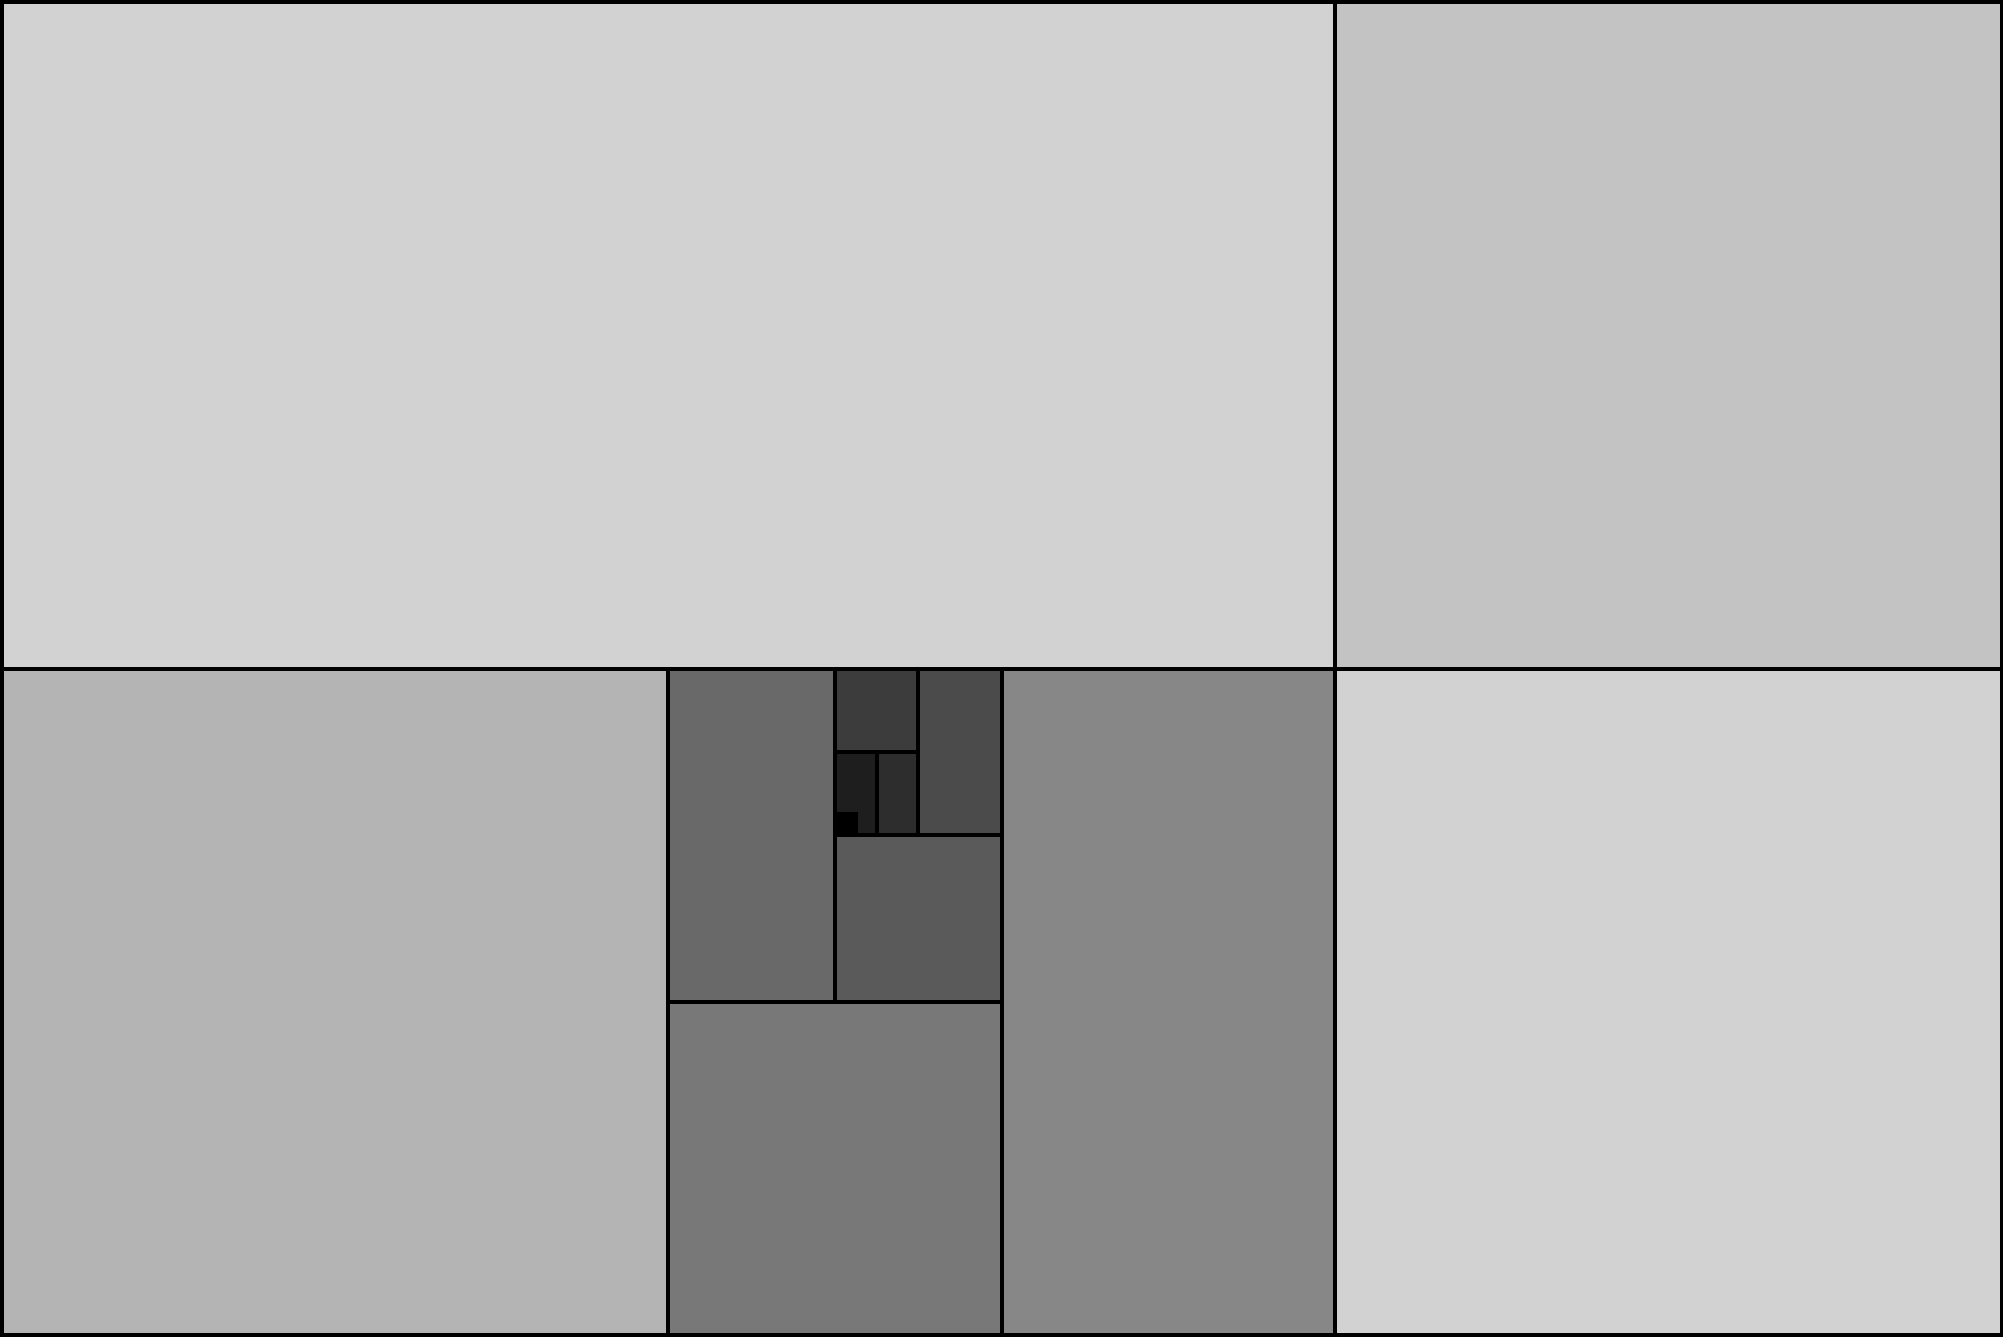
\includegraphics[width=0.8\textwidth]
{trabFinal/direct.pdf}}
\caption{Representa��o esquem�tica de um problema bin�rio resolvido via
algoritmo Direct, onde quanto mais escuro o poliedro formado, melhor o valor da
fun��o objetivo.}
\label{fig:direct}
\end{figure}

O Algoritmo Direct utilizado neste trabalho foi implementado na linguagem
\code{JAVA} dentro do laborat�rio implementando a \emph{Interface}
\code{Objective Function}, presente em \citeonline{ Apache2004}. 

\subsection {Algoritmos estoc�sticos }
A classe de algoritmos estoc�sticos s�o geralmente m�todos de otimiza��o para a
busca do m�nimo global do sistema estudado. O grande diferencial destes m�todos
� a ado��o da aleatoriedade. Esta aleatoriedade conferida ao m�todo d� a
possibilidade de explorar poss�veis solu��es que os algoritmos determin�sticos
como Newton e Nelder Mead n�o proporcionam e geralmente com um n�mero de
itera��es muito menor que m�todos de busca global, como Direct necessitam.

\subsubsection {Algor�tmo Gen�tico (AG)}
O Algoritmo Gen�tico parte da teoria de Charles Darwin, a qual fala que os mais
aptos t�m melhor melhores condi��es de se desenvolver, em contrapartida, os
menos aptos tendem � desaparecer da esp�cie em quest�o, tamb�m conhecida como
sele��o natural. Este m�todo tem por objetivo descartar os piores indiv�duos
(maior valor da fun��o objetivo caso a dire��o seja minimizar a mesma, e
vice-e-versa) e evoluir os melhores. Entretanto, este m�todo � muito dependente
da inicializa��o, uma vez que se a primeira gera��o de indiv�duos � muito ruim,
a probabilidade de que as pr�ximas evoluam para o �timo global n�o � t�o grande
quanto o esperado. Assim, s�o necess�rias v�rias inicializa��es do algoritmo,
selecionando a melhor das melhores.

Este algoritmo foi implementado em \code{JAVA} por \citeonline{Apache2004} e
obtido atrav�s do pacote computacional \code{commons-math-1.2}, dispon�vel na
internet para consulta.

\subsubsection {Particle Swarm Optimization (PSO)}
O m�todo PSO (\emph{Particle Swarm Optimization} -- Optimiza��o por Enxame de
Part�culas) foi implementado na linguagem \code{JAVA} no laborat�rio para fins
deste trabalho. Apresentado por \citeonline{ Kennedy1995}, este m�todo tem duas
principais vertentes, a primeira delas � a vida artificial, representando a
revoada de p�ssaros e cardumes de peixes pela forma do comportamento social
(efeito de madada). A segunda, � inspirada em algoritmos gen�ticos e programa��o
evolucion�ria. Infelizmente, assim como no AG, em que a inicializa��o da rotina
de otimiza��o � aleat�ria, este m�todo depende tamb�m muito de seu in�cio, uma
vez que a melhor part�cula da primeira itera��o coordena o movimento das demais,
fazendo com que sejam necess�rias diversas inicializa��es.


\section{Estima��o dos par�metros}

\subsection{Fun��o objetivo}
Explicar a fun��o objetivo e demonstrar suas equa��es complementares

\subsection{C�digos}
Explicar o que foi implementado e o que j� foi pego pronto de alguma \emph{lib}

 
 
\newdimen\bibindent
\setlength\bibindent{1.5em} {
\rhead{} 
\baselineskip 4.3mm 
\bibliography{bibFinal}}

\end{document}
